\setcounter{section}{20}
\setcounter{subsection}{6}
\setcounter{subsubsection}{0}
% Copyright 2019 by Till Tantau

% This file may be distributed and/or modified

% 1. under the LaTeX Project Public License and/or
% 2. under the GNU Free Documentation License.

% See the file doc/generic/pgf/licenses/LICENSE for more details.


\section{Making Trees Grow\\使树生长}
\label{section-trees}

\subsection{Introduction to the  Child Operation\\引言:Child操作}

\emph{Trees} are a common way of visualizing hierarchical structures. A simple
tree looks like this:

\emph{树}是一种常见的可视化层次结构的方式。一个简单的树看起来像这样:

\begin{codeexample}[]
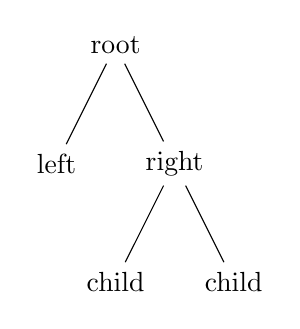
\begin{tikzpicture}
  \node {root}
    child {node {left}}
    child {node {right}
      child {node {child}}
      child {node {child}}
    };
\end{tikzpicture}
\end{codeexample}

Admittedly, in reality trees are more likely to grow \emph{upward} and not
downward as above. You can tell whether the author of a paper is a
mathematician or a computer scientist by looking at the direction their trees
grow. A computer scientist's trees will grow downward while a mathematician's
tree will grow upward. Naturally, the \emph{correct} way is the mathematician's
way, which can be specified as follows:

诚然,实际上树更有可能向\emph{上生长},而不是像上面那样向下生长。通过观察树的生长方向,您可以判断一篇论文的作者是数学家还是计算机科学家。计算机科学家的树会向下生长,而数学家的树会向上生长。当然,\emph{正确}的方式是数学家的方式,可以通过以下方式指定:

\begin{codeexample}[]
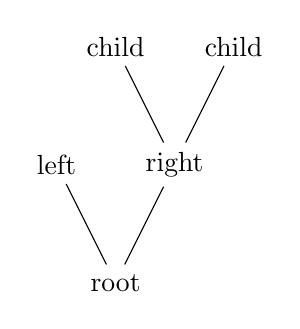
\begin{tikzpicture}
  \node {root} [grow'=up]
    child {node {left}}
    child {node {right}
      child {node {child}}
      child {node {child}}
    };
\end{tikzpicture}
\end{codeexample}

In \tikzname, there are two ways of specifying trees: Using either the |graph|
path operation, which is covered in Section~\ref{section-library-graphs}, or
using the |child| path operation, which is covered in the present section. Both
methods have their advantages.

在 \tikzname\ 中,有两种指定树的方式:使用 |graph| 路径操作,该操作在第~\ref{section-library-graphs}~节中介绍,或者使用 |child| 路径操作,该操作在本节中介绍。这两种方法各有优势。

In \tikzname, trees are specified by adding \emph{children} to a node on a path
using the |child| operation:

在 \tikzname\ 中,通过使用 |child| 操作将\emph{子节点}添加到路径上的节点来指定树:

\begin{pathoperation}{child}{\opt{\oarg{options}}
        \opt{|foreach|\meta{variables}|in|\marg{values}}\opt{\marg{child path}}}
    This operation should directly follow a completed |node| operation or
    another |child| operation, although it is permissible that the first
    |child| operation is preceded by options (we will come to that).

    此操作应该直接跟在一个完成的 |node| 操作或另一个 |child| 操作之后,尽管第一个 |child| 操作之前可以有选项(我们将在后面讨论)。

    When a |node| operation like |node {X}| is followed by |child|, \tikzname\
    starts counting the number of child nodes that follow the original
    |node {X}|. For this, it scans the input and stores away each |child| and
    its arguments until it reaches a path operation that is not a |child|. Note
    that this will fix the character codes of all text inside the child
    arguments, which means, in essence, that you cannot use verbatim text
    inside the nodes inside a |child|. Sorry.

    当像 |node {X}| 这样的 |node| 操作后面跟着 |child| 时,\tikzname\ 开始计算后续的子节点数量,它会扫描输入,并存储每个 |child| 及其参数,直到遇到一个不是 |child| 的路径操作。请注意,这将固定子节点参数内部所有文本的字符编码,这意味着您不能在子节点内部的节点中使用抄录文本。抱歉。

    Once the children have been collected and counted, \tikzname\ starts
    generating the child nodes. For each child of a parent node \tikzname\
    computes an appropriate position where the child is placed. For each child,
    the coordinate system is transformed so that the origin is at this
    position. Then the \meta{child path} is drawn. Typically, the child path
    just consists of a |node| specification, which results in a node being
    drawn at the child's position. Finally, an edge is drawn from the first
    node in the \meta{child path} to the parent node.

    一旦子节点被收集和计数,\tikzname\ 开始生成子节点。对于每个父节点的子节点,\tikzname\ 计算适当的位置来放置子节点。对于每个子节点,坐标系被转换,使得原点位于该位置。然后绘制 \meta{child path}。通常,子路径只包含一个 |node| 规范,这会在子节点的位置绘制一个节点。最后,从 \meta{child path} 中的第一个节点绘制一条边到父节点。

    The optional |foreach| part (note that there is no backslash before
    |foreach|) allows you to specify multiple children in a single |child|
    command. The idea is the following: A |\foreach| statement is (internally)
    used to iterate over the list of \meta{values}. For each value in this
    list, a new |child| is added to the node. The syntax for \meta{variables}
    and for \meta{values} is the same as for the |\foreach| statement, see
    Section~\ref{section-foreach}. For example, when you say
    
    可选的 |foreach| 部分(请注意,在 |foreach| 前面没有反斜杠)允许您在单个 |child| 命令中指定多个子节点。其思想是:内部使用 |\foreach| 语句来迭代 \meta{values} 列表。对于列表中的每个值,都会向节点添加一个新的 |child|。对于 \meta{variables} 和 \meta{values} 的语法与 |\foreach| 语句相同,请参见第~\ref{section-foreach}~节。例如,当您写下

    \begin{codeexample}[code only]
node {root} child [red] foreach \name in {1,2} {node {\name}}
\end{codeexample}
    
    the effect will be the same as if you had said
    
    效果将与您写下以下内容时相同:

    \begin{codeexample}[code only]
node {root} child[red] {node {1}} child[red] {node {2}}
\end{codeexample}
    
    When you write
    
    当您写下

    \begin{codeexample}[code only]
node {root} child[\pos] foreach \name/\pos in {1/left,2/right} {node[\pos] {\name}}
\end{codeexample}
    
    the effect will be the same as for
    
    效果与下面的相同

    \begin{codeexample}[code only]
node {root} child[left] {node[left] {1}} child[right] {node[right] {2}}
\end{codeexample}

    You can nest things as in the following example:
    
    您可以像以下示例中一样嵌套使用:

    \begin{codeexample}[]
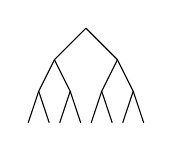
\begin{tikzpicture}
  [level distance=4mm,level/.style={sibling distance=8mm/#1}]
  \coordinate
    child foreach \x in {0,1}
      {child foreach \y in {0,1}
        {child foreach \z in {0,1}}};
\end{tikzpicture}
\end{codeexample}

    The details and options for this operation are described in the rest of
    this present section.

    此操作的详细信息和选项在本节的其余部分中描述。

  \end{pathoperation}


\subsection{Child Paths and Child Nodes\\子路径和子节点}

For each |child| of a root node, its \meta{child path} is inserted at a
specific location in the picture (the placement rules are discussed in
Section~\ref{section-tree-placement}). The first node in the \meta{child path},
if it exists, is special and called the \emph{child node}. If there is no first
node in the \meta{child path}, that is, if the \meta{child path} is missing
(including the curly braces) or if it does not start with |node| or with
|coordinate|, then an empty child node of shape |coordinate| is automatically
added.

对于根节点的每个|child|,它的\meta{child path}被插入到图中的特定位置(放置规则在第~\ref{section-tree-placement}节中讨论)。\meta{child path}中的第一个节点(如果存在)是特殊的,称为\emph{子节点}。如果\meta{child path}中没有第一个节点,即\meta{child path}丢失(包括花括号)或者不以|node|或|coordinate|开头,那么将自动添加一个形状为|coordinate|的空子节点。

Consider the example |\node {x} child {node {y}} child;|. For the first child,
the \meta{child path} has the child node |node {y}|. For the second child, no
child node is specified and, thus, it is just |coordinate|.

考虑示例|\node {x} child {node {y}} child;|。对于第一个子节点,\meta{child path}具有子节点|node {y}|。对于第二个子节点,未指定子节点,因此只是|coordinate|。

As for any normal node, you can give the child node a name, shift it around, or
use options to influence how it is rendered.

对于任何普通节点一样,您可以给子节点命名,对其进行平移,或使用选项来影响其渲染方式。

\begin{codeexample}[preamble={\usetikzlibrary{shapes.geometric}}]
\begin{tikzpicture}[sibling distance=15mm]
  \node[rectangle,draw] {root}
    child {node[circle,draw,yshift=-5mm] (left node) {left}}
    child {node[ellipse,draw] (right node) {right}};
  \draw[dashed,->] (left node) -- (right node);
\end{tikzpicture}
\end{codeexample}

In many cases, the \meta{child path} will just consist of a specification of a
child node and, possibly, children of this child node. However, the node
specification may be followed by arbitrary other material that will be added to
the picture, transformed to the child's coordinate system. For your
convenience, a move-to |(0,0)| operation is inserted automatically at the
beginning of the path. Here is an example:

在许多情况下,\meta{child path}只是一个子节点的规范,可能还有这个子节点的子节点。然而,节点规范后面可能跟随任意其他材料,将其添加到子节点的坐标系中。为了方便起见,将自动在路径的开头插入一个移动到|(0,0)|的操作。以下是一个示例:

\begin{codeexample}[]
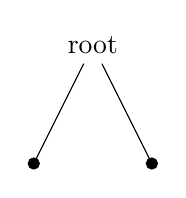
\begin{tikzpicture}
  \node {root}
    child {[fill] circle (2pt)}
    child {[fill] circle (2pt)};
\end{tikzpicture}
\end{codeexample}

At the end of the \meta{child path} you may add a special path operation called
|edge from parent|. If this operation is not given by yourself somewhere on the
path, it will be automatically added at the end. This option causes a
connecting edge from the parent node to the child node to be added to the path.
By giving options to this operation you can influence how the edge is rendered.
Also, nodes following the |edge from parent| operation will be placed on this
edge, see Section~\ref{section-edge-from-parent} for details.

在\meta{child path}的末尾,您可以添加一个名为|edge from parent|的特殊路径操作。如果在路径的某个位置没有指定此操作,它将自动添加到末尾。此选项会在路径中添加从父节点到子节点的连接边。通过给此操作添加选项,可以影响边的渲染方式。此外,跟随|edge from parent|操作的节点将放置在此边上,请参阅第~\ref{section-edge-from-parent}节了解详细信息。

To sum up:

总结一下:

\begin{enumerate}
    \item The child path starts with a node specification. If it is not there,
        it is added automatically.

        子路径以节点规范开头。如果不存在,则会自动添加。


    \item The child path ends with a |edge from parent| operation, possibly
        followed by nodes to be put on this edge. If the operation is not given
        at the end, it is added automatically.

        子路径以|edge from parent|操作结束,可能后面跟随要放置在此边上的节点。如果未在末尾给出该操作,则会自动添加。

      \end{enumerate}


\subsection{Naming Child Nodes\\命名子节点}

Child nodes can be named like any other node using either the |name| option or
the special syntax in which the name of the node is placed in round parentheses
between the |node| operation and the node's text.

子节点可以像其他节点一样使用 |name| 选项或特殊语法进行命名,特殊语法是将节点的名称放置在 |node| 操作和节点的文本之间的圆括号中。

If you do not assign a name to a child node, \tikzname\ will automatically
assign a name as follows: Assume that the name of the parent node is, say,
|parent|. (If you did not assign a name to the parent, \tikzname\ will do so
itself, but that name will not be user-accessible.) The first child of |parent|
will be named |parent-1|, the second child is named |parent-2|, and so on.

如果不为子节点分配名称,\tikzname\ 将自动分配名称,如下所示:假设父节点的名称是 |parent|。(如果您没有为父节点分配名称,\tikzname\ 将自动分配名称,但该名称将无法通过用户访问。)第一个子节点的名称是 |parent-1|,第二个子节点的名称是 |parent-2|,依此类推。

This naming convention works recursively. If the second child |parent-2| has
children, then the first of these children will be called |parent-2-1| and the
second |parent-2-2| and so on.

此命名约定递归地起作用。如果第二个子节点 |parent-2| 有子节点,则第一个子节点将被称为 |parent-2-1|,第二个子节点将被称为 |parent-2-2|,依此类推。

If you assign a name to a child node yourself, no name is generated
automatically (the node does not have two names). However, ``counting
continues'', which means that the third child of |parent| is called |parent-3|
independently of whether you have assigned names to the first and/or second
child of |parent|.

如果您自己为子节点分配了名称,则不会自动生成名称(节点不会有两个名称)。但是,``计数会继续'',这意味着无论您是否为 |parent| 的第一个和/或第二个子节点分配了名称,第三个子节点都被称为 |parent-3|。

Here is an example:

以下是一个示例:

\begin{codeexample}[]
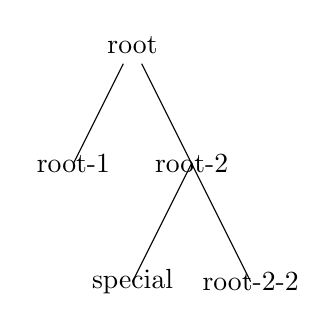
\begin{tikzpicture}[sibling distance=15mm]
  \node (root) {root}
    child
    child {
      child {coordinate (special)}
      child
    };
  \node at (root-1) {root-1};
  \node at (root-2) {root-2};
  \node at (special) {special};
  \node at (root-2-2) {root-2-2};
\end{tikzpicture}
\end{codeexample}


\subsection{Specifying Options for Trees and Children\\为树和子节点指定选项}
\label{section-tree-options}

Each |child| may have its own \meta{options}, which apply to ``the whole
child'', including all of its grandchildren. Here is an example:

每个 |child| 可以具有自己的 \meta{options},这些选项适用于``整个子节点'',包括其所有的孙节点。以下是一个示例:

\begin{codeexample}[]
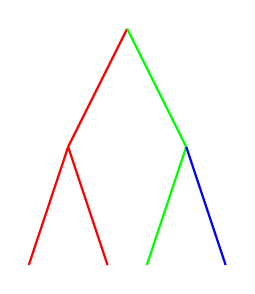
\begin{tikzpicture}
  [thick,level 1/.style={sibling distance=15mm},
         level 2/.style={sibling distance=10mm}]
  \coordinate
    child[red]   {child child}
    child[green] {child child[blue]};
\end{tikzpicture}
\end{codeexample}

The options of the root node have no effect on the children since the options
of a node are always ``local'' to that node. Because of this, the edges in the
following tree are black, not red.

根节点的选项对子节点没有影响,因为节点的选项始终是对该节点``局部''的。因此,以下树中的边是黑色的,而不是红色的。

\begin{codeexample}[]
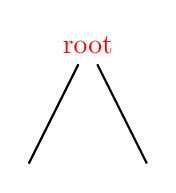
\begin{tikzpicture}[thick]
  \node [red] {root}
    child
    child;
\end{tikzpicture}
\end{codeexample}

This raises the problem of how to set options for \emph{all} children.
Naturally, you could always set options for the whole path as in
|\path [red] node {root} child child;| but this is bothersome in some
situations. Instead, it is easier to give the options \emph{before the first
child} as follows: 

这引发了如何为\emph{所有}子节点设置选项的问题。当然,您可以始终对整个路径设置选项,如 |\path [red] node {root} child child;|,但在某些情况下这可能很麻烦。相反,更容易的方法是在第一个子节点之前给出选项,如下所示:

\begin{codeexample}[]
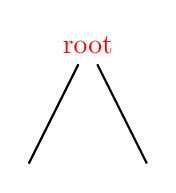
\begin{tikzpicture}[thick]
\node [red] {root}%
%[green] option applies to all children%
child%
child;
\end{tikzpicture}
\end{codeexample}

Here is the set of rules:

以下是一组规则:

\begin{enumerate}
    \item Options for the whole tree are given before the root node.

    树的整体选项位于根节点之前。


    \item Options for the root node are given directly to the |node| operation
        of the root.
   
        根节点的选项直接给出给根节点的 |node| 操作。

        \item Options for all children can be given between the root node and the
        first child.

        所有子节点的选项可以在根节点和第一个子节点之间给出。

        \item Options applying to a specific child path are given as options to the
        |child| operation.

        适用于特定子节点路径的选项作为 |child| 操作的选项给出。

        \item Options applying to the node of a child, but not to the whole child
        path, are given as options to the |node| command inside the \meta{child
        path}.

        适用于子节点的节点(但不适用于整个子节点路径)的选项作为 |node| 命令中的选项给出,位于 \meta{child path} 内部。


\end{enumerate}

\begin{codeexample}[code only]
\begin{tikzpicture}
  \scoped
    [...]              Options apply to the whole tree
    \node[...] {root}  Options apply to the root node only
       [...]           Options apply to all children
       child[...]      Options apply to this child and all its children
       {
         node[...] {}  Options apply to the child node only
         ...
       }
       child[...]      Options apply to this child and all its children
    ;
\end{tikzpicture}
\end{codeexample}

There are additional styles that influence how children are rendered:

还有其他样式会影响子节点的呈现:

\begin{stylekey}{/tikz/every child (initially \normalfont empty)}
    This style is used at the beginning of each child, as if you had given the
    style's contents as options to the |child| operation.

    此样式在每个子节点的开头使用,就像将样式内容作为 |child| 操作的选项一样。

  \end{stylekey}

\begin{stylekey}{/tikz/every child node (initially \normalfont empty)}
    This style is used at the beginning of each child node in addition to the
    |every node| style.

    此样式除了 |every node| 样式之外,还在每个子节点的开头使用。

  \end{stylekey}

\begin{stylekey}{/tikz/level=\meta{number} (initially \normalfont empty)}
    This style is executed at the beginning of each set of children, where
    \meta{number} is the current level in the current tree. For example, when
    you say |\node {x} child child;|, then |level=1| is used before the first
    |child|. The style or code of this key will be passed \meta{number} as its
    first parameter. If this first |child| has children itself, then |level=2|
    would be used for them.
    
    此样式在每个子节点集的开头执行,其中 \meta{number} 是当前树中的当前级别。例如,当您说 |\node {x} child child;| 时,将在第一个 |child| 之前使用 |level=1|。此键的样式或代码将使用 \meta{number} 作为其第一个参数。如果此第一个 |child| 本身有子节点,则对它们使用 |level=2|。

    \begin{codeexample}[]
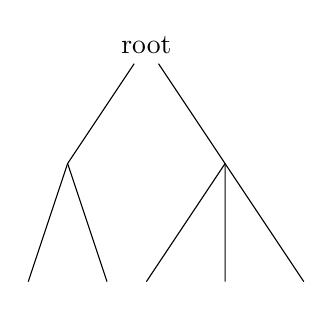
\begin{tikzpicture}[level/.style={sibling distance=20mm/#1}]
  \node {root}
    child { child child }
    child { child child child };
\end{tikzpicture}
\end{codeexample}
    
\end{stylekey}

\begin{stylekey}{/tikz/level \meta{number} (initially \normalfont empty)}
    This style is used in addition to the |level| style. So, when you say
    |\node {x} child child;|, then the following key list is executed:
    |level=1,level 1|.
    
    此样式除了 |level| 样式外还会使用。因此,当您说 |\node {x} child child;| 时,将执行以下键列表:|level=1,level 1|。

    \begin{codeexample}[]
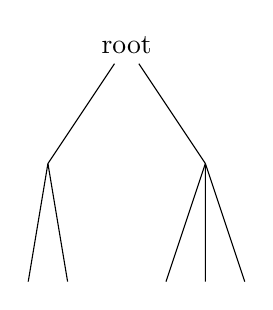
\begin{tikzpicture}
  [level 1/.style={sibling distance=20mm},
   level 2/.style={sibling distance=5mm}]
  \node {root}
    child { child child }
    child { child child child };
\end{tikzpicture}
\end{codeexample}
    
\end{stylekey}


\subsection{Placing Child Nodes\\放置子节点}
\label{section-tree-placement}

\subsubsection{Basic Idea\\基本思路}

Perhaps the most difficult part in drawing a tree is the correct layout of the
children. Typically, the children have different sizes and it is not easy to
arrange them in such a manner that not too much space is wasted, the children
do not overlap, and they are either evenly spaced or their centers are evenly
distributed. Calculating good positions is especially difficult since a good
position for the first child may depend on the size of the last child.

绘制树形结构中最困难的部分也许是正确布局子节点。通常,子节点的大小不同,并不容易将它们排列在不浪费太多空间、不重叠且均匀间隔或其中心均匀分布的方式。计算良好的位置尤其困难,因为第一个子节点的良好位置可能取决于最后一个子节点的大小。

In basic \tikzname, when you do not make use of the graph drawing facilities
explained in Part~\ref{part-gd}, a comparatively simple approach is taken to
placing the children. In order to compute a child's position, all that is taken
into account is the number of the current child in the list of children and the
number of children in this list. Thus, if a node has five children, then there
is a fixed position for the first child, a position for the second child, and
so on. These positions \emph{do not depend on the size of the children} and,
hence, children can easily overlap. However, since you can use options to shift
individual children a bit, this is not as great a problem as it may seem.

在基本的\tikzname 中,当您不使用在第\ref{part-gd}部分中介绍的图绘制功能时,放置子节点采用了相对简单的方法。为了计算子节点的位置,只考虑了子节点在子节点列表中的编号和子节点列表中的子节点数。因此,如果一个节点有五个子节点,那么第一个子节点有一个固定的位置,第二个子节点有一个位置,依此类推。这些位置\emph{不依赖于子节点的大小},因此子节点可能会重叠。然而,由于您可以使用选项略微移动单个子节点,因此这并不是一个大问题。

Although the placement of the children only depends on their number in the list
of children and the total number of children, everything else about the
placement is highly configurable. You can change the distance between children
(appropriately called the |sibling distance|) and the distance between levels
of the tree. These distances may change from level to level. The direction in
which the tree grows can be changed globally and for parts of the tree. You can
even specify your own ``growth function'' to arrange children on a circle or
along special lines or curves.

尽管子节点的放置仅取决于它们在子节点列表中的编号和子节点的总数,但有关放置的其他所有内容都是高度可配置的。您可以更改子节点之间的距离(适当称为|sibling distance|)以及树的层级之间的距离。这些距离可能会在不同层级之间发生变化。可以全局和局部更改树生长的方向。甚至可以指定自己的“生长函数”以便将子节点排列在圆上或沿着特定的线条或曲线上。


\subsubsection{Default Growth Function\\默认的生长函数}

The default growth function works as follows: Assume that we are given a node
and five children. These children will be placed on a line with their centers
(or, more generally, with their anchors) spaced apart by the current
|sibling distance|. The line is orthogonal to the current \emph{direction of
growth}, which is set with the |grow| and |grow'| option (the latter option
reverses the ordering of the children). The distance from the line to the
parent node is given by the |level distance|.

默认的生长函数工作方式如下:假设我们给定一个节点和五个子节点。这些子节点将在一条线上排列,它们的中心(或更一般地说,它们的锚点)之间的间隔由当前的|sibling distance|确定。该线与当前的\emph{生长方向}垂直,该方向由|grow|和|grow'|选项设置(后一选项颠倒了子节点的顺序)。从线到父节点的距离由|level distance|给出。

{\catcode`\|=12
\begin{codeexample}[]
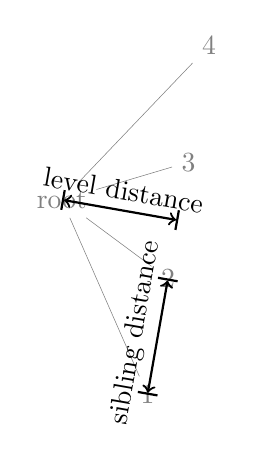
\begin{tikzpicture}[sibling distance=15mm, level distance=15mm]
  \path [help lines]
    node (root) {root}
    [grow=-10]
    child {node {1}}
    child {node {2}}
    child {node {3}}
    child {node {4}};

  \draw[|<->|,thick] (root-1.center)
    -- node[above,sloped] {sibling distance} (root-2.center);

  \draw[|<->|,thick] (root.center)
    -- node[above,sloped] {level distance} +(-10:\tikzleveldistance);
\end{tikzpicture}
\end{codeexample}
}

\begin{key}{/tikz/level distance=\meta{distance} (initially 15mm)}
    This key determines the distance between different levels of the tree, more
    precisely, between the parent and the line on which its children are
    arranged. When given to a single child, this will set the distance for this
    child only.

    此键确定树的不同层级之间的距离,更准确地说,确定父节点与其子节点排列所在的线之间的距离。当应用于单个子节点时,仅设置该子节点的距离。
\begin{codeexample}[]
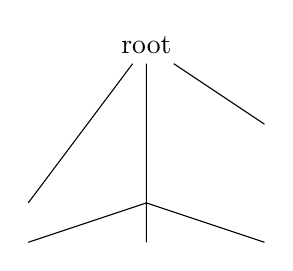
\begin{tikzpicture}
  \node {root}
    [level distance=20mm]
    child
    child {
      [level distance=5mm]
      child
      child
      child
    }
    child[level distance=10mm];
\end{tikzpicture}
\end{codeexample}

\begin{codeexample}[]
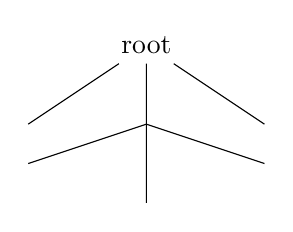
\begin{tikzpicture}
  [level 1/.style={level distance=10mm},
   level 2/.style={level distance=5mm}]
  \node {root}
    child
    child {
      child
      child[level distance=10mm]
      child
    }
    child;
\end{tikzpicture}
\end{codeexample}
    
\end{key}

\begin{key}{/tikz/sibling distance=\meta{distance} (initially 15mm)}
    This key specifies the distance between the anchors of the children of a
    parent node.
    
    此键指定父节点的子节点之间的距离。

    \begin{codeexample}[]
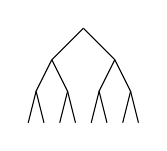
\begin{tikzpicture}
  [level distance=4mm,
   level 1/.style={sibling distance=8mm},
   level 2/.style={sibling distance=4mm},
   level 3/.style={sibling distance=2mm}]
  \coordinate
     child {
       child {child child}
       child {child child}
     }
     child {
       child {child child}
       child {child child}
     };
\end{tikzpicture}
\end{codeexample}

\begin{codeexample}[]
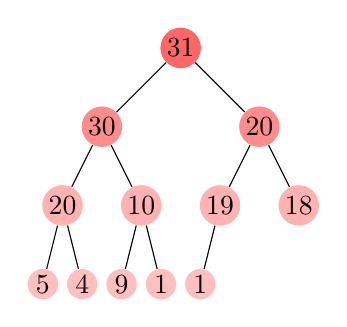
\begin{tikzpicture}
  [level distance=10mm,
   every node/.style={fill=red!60,circle,inner sep=1pt},
   level 1/.style={sibling distance=20mm,nodes={fill=red!45}},
   level 2/.style={sibling distance=10mm,nodes={fill=red!30}},
   level 3/.style={sibling distance=5mm,nodes={fill=red!25}}]
  \node {31}
     child {node {30}
       child {node {20}
         child {node {5}}
         child {node {4}}
       }
       child {node {10}
         child {node {9}}
         child {node {1}}
       }
     }
     child {node {20}
       child {node {19}
         child {node {1}}
         child[missing]
       }
       child {node {18}}
     };
\end{tikzpicture}
\end{codeexample}
    
\end{key}

\begin{key}{/tikz/grow=\meta{direction}}
    This key is used to define the \meta{direction} in which the tree will
    grow. The \meta{direction} can either be an angle in degrees or one of the
    following special text strings: |down|, |up|, |left|, |right|, |north|,
    |south|, |east|, |west|, |north east|, |north west|, |south east|, and
    |south west|. All of these have ``their obvious meaning'', so, say,
    |south west| is the same as the angle $-135^\circ$.

    此键用于定义树生长的\meta{direction}。这里的\meta{direction}可以是角度(以度为单位),也可以是以下特殊文本字符串之一:|down|、|up|、|left|、|right|、|north|、|south|、|east|、|west|、|north east|、|north west|、|south east|和|south west|。所有这些都有“显而易见的含义”,因此,例如,|south west|与角度$-135^\circ$相同。

    As a side effect, this option installs the default growth function.

    作为副作用,该选项安装了默认的增长函数。



    

    In addition to setting the direction, this option also has a seemingly
    strange effect: It sets the sibling distance for the current level to
    |0pt|, but leaves the sibling distance for later levels unchanged.

    作为副作用,此选项还具有一种看似奇怪的效果:它将当前级别的子节点距离设置为|0pt|,但保持后续级别的子节点距离不变。



    This somewhat strange behavior has a highly desirable effect: If you give
    this option before the list of children of a node starts, the ``current
    level'' is still the parent level. Each child will be on a later level and,
    hence, the sibling distance will be as specified originally. This will
    cause the children to be neatly aligned in a line orthogonal to the given
    \meta{direction}. However, if you give this option locally to a single
    child, then ``current level'' will be the same as the child's level. The
    zero sibling distance will then cause the child to be placed exactly at a
    point at distance |level distance| in the direction \meta{direction}.
    However, the children of the child will be placed ``normally'' on a line
    orthogonal to the \meta{direction}.

    
    这种稍微奇怪的行为有一个非常理想的效果:如果您在节点的子节点列表开始之前给出此选项,那么当前级别''仍然是父级别。每个子节点将在后续级别上,因此同级距离将如最初指定的那样。这将导致子节点在与给定的 \meta{direction} 正交的线上整齐对齐。然而,如果您将此选项局部地应用于单个子节点,则当前级别''将与子级别相同。零同级距离将导致将子节点精确地放置在距离为 |level distance| 的点上,该点位于 \meta{direction} 方向上。然而,子节点的子节点将``正常''地放置在与 \meta{direction} 正交的线上。


    These placement effects are best demonstrated by some examples:

    这些放置效果最好通过一些示例来演示:
    
\begin{codeexample}[]
\tikz \node {root} [grow=right] child child;
\end{codeexample}

\begin{codeexample}[]
\tikz \node {root} [grow=south west] child child;
\end{codeexample}

\begin{codeexample}[]
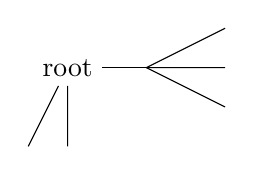
\begin{tikzpicture}[level distance=10mm,sibling distance=5mm]
  \node {root}
    [grow=down]
    child
    child
    child[grow=right] {
      child child child
    };
\end{tikzpicture}
\end{codeexample}

\begin{codeexample}[]
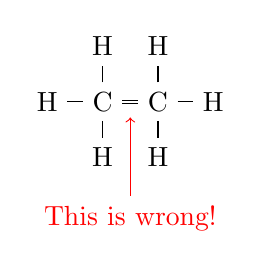
\begin{tikzpicture}[level distance=2em]
  \node {C}
    child[grow=up]    {node {H}}
    child[grow=left]  {node {H}}
    child[grow=down]  {node {H}}
    child[grow=right] {node {C}
        child[grow=up]    {node {H}}
        child[grow=right] {node {H}}
        child[grow=down]  {node {H}}
      edge from parent[double]
        coordinate (wrong)
    };
  \draw[<-,red] ([yshift=-2mm]wrong) -- +(0,-1)
    node[below]{This is wrong!};
\end{tikzpicture}
\end{codeexample}

\begin{codeexample}[]
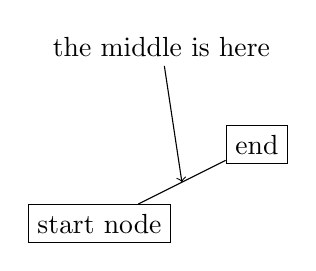
\begin{tikzpicture}
  \node[rectangle,draw] (a) at (0,0) {start node};
  \node[rectangle,draw] (b) at (2,1) {end};

  \draw (a) -- (b)
    node[coordinate,midway] {}
      child[grow=100,<-] {node[above] {the middle is here}};
\end{tikzpicture}
\end{codeexample}
    
\end{key}

\begin{key}{/tikz/grow'=\meta{direction}}
    This key has the same effect as |grow|, only the children are arranged in
    the opposite order.

    此键与|grow|具有相同的效果,只是子节点的排列顺序相反。


\end{key}


\subsubsection{Missing Children\\缺失的子节点}

Sometimes one or more of the children of a node are ``missing''. Such a missing
child will count as a child with respect to the total number of children and
also with respect to the current child count, but it will not be rendered.

有时一个或多个节点的子节点是“缺失”的。这样的缺失子节点在总子节点数和当前子节点计数方面都被计算在内,但不会被渲染。

\begin{key}{/tikz/missing=\meta{true or false} (default true)}
    If this option is given to a child, the current child counter is increased,
    but the child is otherwise ignored. In particular, the normal contents of
    the child is completely ignored.
    
    如果给子节点设置了此选项,则当前子节点计数会增加,但子节点会被忽略。特别地,子节点的正常内容将完全被忽略。

    \begin{codeexample}[]
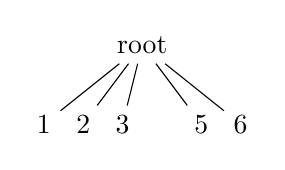
\begin{tikzpicture}[level distance=10mm,sibling distance=5mm]
  \node {root} [grow=down]
    child          { node {1} }
    child          { node {2} }
    child          { node {3} }
    child[missing] { node {4} }
    child          { node {5} }
    child          { node {6} };
\end{tikzpicture}
\end{codeexample}
    
\end{key}


\subsubsection{Custom Growth Functions\\自定义生长函数}

\begin{key}{/tikz/growth parent anchor=\meta{anchor} (initially center)}
    This key allows you to specify which anchor of the parent node is to be
    used for computing the children's position. For example, when there is only
    one child and the |level distance| is |2cm|, then the child node will be
    placed two centimeters below the \meta{anchor} of the parent node. ``Being
    placed'' means that the child node's anchor (which is the anchor specified
    using the |anchor=| option in the |node| command of the child) is two
    centimeters below the parent node's \meta{anchor}.

    该键允许您指定父节点的哪个锚点用于计算子节点的位置。例如,当只有一个子节点且 |level distance| 为 |2cm| 时,子节点将被放置在父节点的 \meta{anchor} 下方两厘米处。“被放置”意味着子节点的锚点(使用子节点的 |node| 命令中的 |anchor=| 选项指定的锚点)在父节点的 \meta{anchor} 下方两厘米。

    In the following example, the two red lines both have length |1cm|.
    
    在下面的示例中,两个红线的长度都为 |1cm|。

    \begin{codeexample}[]
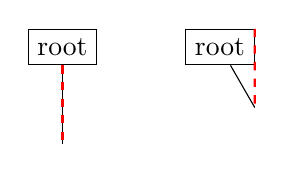
\begin{tikzpicture}[level distance=1cm]
  \node [rectangle,draw] (a) at (0,0) {root}
  [growth parent anchor=south] child;

  \node [rectangle,draw] (b) at (2,0) {root}
  [growth parent anchor=north east] child;

  \draw [red,thick,dashed] (a.south) -- (a-1);
  \draw [red,thick,dashed] (b.north east) -- (b-1);
\end{tikzpicture}
\end{codeexample}

    In the next example, the top and bottom nodes are aligned at the top and
    the bottom, respectively.
    
    在下一个示例中,顶部和底部节点分别与顶部和底部对齐。

    \begin{codeexample}[]
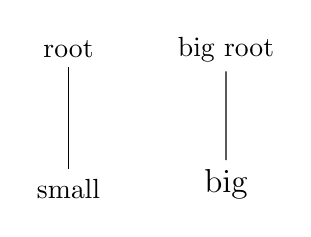
\begin{tikzpicture}
  [level distance=2cm,growth parent anchor=north,
   every node/.style={anchor=north,rectangle,draw}
   every child node/.style={anchor=south}]

  \node at (0,0) {root} child {node {small}};

  \node at (2,0) {big root} child {node {\large big}};
\end{tikzpicture}
\end{codeexample}
    
\end{key}

\begin{key}{/tikz/growth function=\meta{macro name} (initially \normalfont an internal function)}
    This rather low-level option allows you to set a new growth function. The
    \meta{macro name} must be the name of a macro without parameters. This
    macro will be called for each child of a node. The initial function is an
    internal function that corresponds to downward growth.

    这个相当底层的选项允许您设置一个新的生长函数。 \meta{macro name} 必须是一个无参数的宏的名称。对于每个节点的子节点,都会调用此宏。初始函数是一个对应于向下生长的内部函数。

    The effect of executing the macro should be the following: It should
    transform the coordinate system in such a way that the origin becomes the
    place where the current child should be anchored. When the macro is called,
    the current coordinate system will be set up such that the anchor of the
    parent node is in the origin. Thus, in each call, the \meta{macro name}
    must essentially do a shift to the child's origin. When the macro is
    called, the \TeX\ counter |\tikznumberofchildren| will be set to the total
    number of children of the parent node and the counter
    |\tikznumberofcurrentchild| will be set to the number of the current child.

    执行宏的效果应该是:它应该以一种方式转换坐标系,使得原点成为当前子节点应锚定的位置。当调用宏时,当前坐标系将被设置,以使父节点的锚点位于原点。因此,在每次调用时,\meta{macro name} 实际上必须对子节点的原点进行移动。在调用宏时,\TeX 计数器 |\tikznumberofchildren| 将被设置为父节点的子节点总数,计数器 |\tikznumberofcurrentchild| 将被设置为当前子节点的编号。

    The macro may, in addition to shifting the coordinate system, also
    transform the coordinate system further. For example, it could be rotated
    or scaled.

    除了移动坐标系,宏还可以进一步变换坐标系。例如,可以进行旋转或缩放。

    Additional growth functions are defined in the library, see
    Section~\ref{section-tree-library}.

    库中定义了其他的生长函数,请参见第~\ref{section-tree-library} 节。

  \end{key}


\subsection{Edges From the Parent Node\\从父节点出发的边缘}
\label{section-edge-from-parent}

Every child node is connected to its parent node via a special kind of edge
called the |edge from parent|. This edge is added to the \meta{child path} when
the following path operation is encountered:

每个子节点通过一种称为 |edge from parent| 的特殊类型的边缘连接到其父节点。当遇到以下路径操作时,这个边缘将被添加到 \meta{child path} 中:

\begin{pathoperation}{edge from parent}{\opt{\oarg{options}}}
    This path operation can only be used inside \meta{child paths} and should
    be given at the end, possibly followed by \meta{node specifications} like
    |node {a}|. If a \meta{child path} does not contain this operation, it will
    be added at the end of the \meta{child path} automatically.

    此路径操作只能在 \meta{child paths} 中使用,并且应该在结尾处给出,可能后面跟着 \meta{node specifications},如 |node {a}|。如果一个 \meta{child path} 不包含此操作,它将在 \meta{child path} 的末尾自动添加。

    By default, this operation does the following:
    
    默认情况下,此操作执行以下操作:

    \begin{enumerate}
        \item The following style is executed:
            
        执行以下样式:


            \begin{stylekey}{/tikz/edge from parent (initially draw)}
                This style is inserted right before the |edge from parent path|
                and before the \meta{options} are inserted.
                
                此样式插入到 |edge from parent path| 之前,并在插入 \meta{options} 之前。


\begin{codeexample}[]
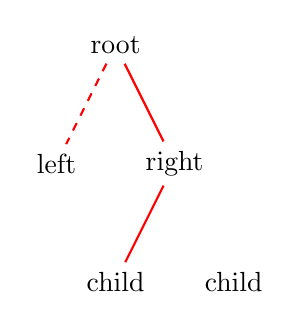
\begin{tikzpicture}
  [edge from parent/.style={draw,red,thick}]
  \node {root}
    child {node {left} edge from parent[dashed]}
    child {node {right}
      child {node {child}}
      child {node {child} edge from parent[draw=none]}
    };
\end{tikzpicture}
\end{codeexample}
            \end{stylekey}
        \item Next, the \meta{options} are executed.

        然后,执行 \meta{options}。


        \item Next, the text stored in the following key is inserted:
            
        接下来,插入以下键中存储的文本:


            \begin{key}{/tikz/edge from parent path=\meta{path} (initially \normalfont code shown below)}
                This option allows you to set the |edge from parent path| to a
                new path. Initially, this path is the following:
                
                这个选项允许您将 |edge from parent path| 设置为一个新的路径。初始情况下,此路径如下:


\begin{codeexample}[code only]
(\tikzparentnode\tikzparentanchor) -- (\tikzchildnode\tikzchildanchor)
\end{codeexample}
                
                The |\tikzparentnode| is a macro that will expand to the name
                of the parent node. This works even when you have not assigned
                a name to the parent node, in this case an internal name is
                automatically generated. The |\tikzchildnode| is a macro that
                expands to the name of the child node. The two |...anchor|
                macros are empty by default. So, what is essentially inserted
                is just the path segment
                |(\tikzparentnode) -- (\tikzchildnode)|; which is exactly an
                edge from the parent to the child.

                |\tikzparentnode| 是一个宏,它将展开为父节点的名称。即使您没有为父节点分配名称,这也可以工作,此时将自动生成一个内部名称。|\tikzchildnode| 是一个宏,它展开为子节点的名称。两个 |...anchor| 宏默认为空。因此,实际插入的内容只是路径段 |(\tikzparentnode) -- (\tikzchildnode)|;这恰好是从父节点到子节点的边。

                You can modify this edge from parent path to achieve all sorts
                of effects. For example, we could replace the straight line by
                a curve as follows:

                您可以修改此 |edge from parent path| 以实现各种效果。例如,我们可以将直线替换为曲线,如下所示:


\begin{codeexample}[]
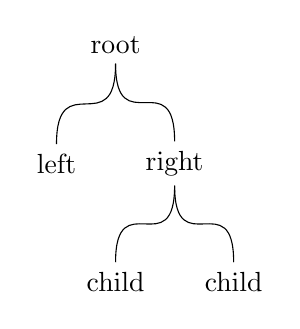
\begin{tikzpicture}[level distance=15mm, sibling distance=15mm,
  edge from parent path=
  {(\tikzparentnode.south) .. controls +(0,-1) and +(0,1)
                           .. (\tikzchildnode.north)}]
  \node {root}
    child {node {left}}
    child {node {right}
      child {node {child}}
      child {node {child}}
    };
\end{tikzpicture}
\end{codeexample}

                Further useful |edge from parent path|s are defined in the tree
                library, see Section~\ref{section-tree-library}.

                更多有用的 |edge from parent path| 在树库中定义,参见第~\ref{section-tree-library} 节。

                The nodes in a \meta{node specification} following the
                |edge from parent| path command get executed as if the |pos|
                option had been added to all these nodes, see also
                Section~\ref{section-pos-option}.

                在 |edge from parent| 路径命令之后的 \meta{node specification} 中的节点将执行,就好像在所有这些节点中添加了 |pos| 选项一样,参见第~\ref{section-pos-option} 节。

                As an example, consider the following code:

                例如,考虑以下代码:


\begin{codeexample}[code only]
\node (root) {} child {node (child) {} edge to parent node {label}};
\end{codeexample}
                
                The |edge to parent| operation and the following |node|
                operation will, together, have the same effect as if we had
                said:
                
                |edge to parent| 操作和随后的 |node| 操作将一起产生与下面的代码相同的效果:


\begin{codeexample}[code only]
(root) -- (child) node [pos=0.5] {label}
\end{codeexample}

                Here is a more complicated example:
                
                以下是一个更复杂的示例:


\begin{codeexample}[]
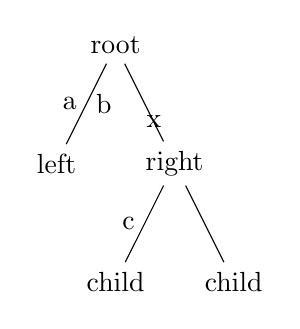
\begin{tikzpicture}
  \node {root}
    child {
      node {left}
      edge from parent
        node[left] {a}
        node[right] {b}
    }
    child {
      node {right}
        child {
          node {child}
          edge from parent
            node[left] {c}
        }
        child {node {child}}
      edge from parent
        node[near end] {x}
    };
\end{tikzpicture}
\end{codeexample}

                As said before, the anchors in the default
                |edge from parent path| are empty. However, you can set them
                using the following keys:
                
                如前所述,默认的 |edge from parent path| 中的锚点为空。但是,您可以使用以下键设置它们:

                \begin{key}{/tikz/child anchor=\meta{anchor} (initially border)}
                    Specifies the anchor where the edge from parent meets the
                    child node by setting the macro |\tikzchildanchor| to
                    |.|\meta{anchor}.

                    通过将宏 |\tikzchildanchor| 设置为 |.|\meta{anchor},指定了从父节点到子节点的边所连接的锚点。

                    If you specify |border| as the \meta{anchor}, then the
                    macro |\tikzchildanchor| is set to the empty string. The
                    effect of this is that the edge from the parent will meet
                    the child on the border at an automatically calculated
                    position.
                    
                    如果将 \meta{anchor} 指定为 |border|,则宏 |\tikzchildanchor| 将设置为空字符串。其效果是,从父节点到子节点的边将在自动计算的位置处在边界上相交。

                    \begin{codeexample}[]
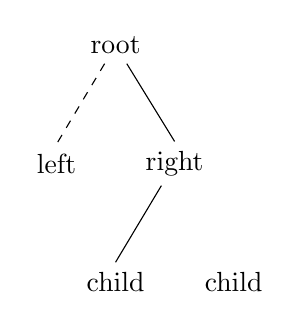
\begin{tikzpicture}
  \node {root}
    [child anchor=north]
    child {node {left} edge from parent[dashed]}
    child {node {right}
      child {node {child}}
      child {node {child} edge from parent[draw=none]}
    };
\end{tikzpicture}
\end{codeexample}
                \end{key}

                \begin{key}{/tikz/parent anchor=\meta{anchor} (initially border)}
                    This option works the same way as the |child anchor|, only
                    for the parent.

                    该选项与 |child anchor| 的工作方式相同,只是针对父节点。


                \end{key}
            \end{key}
    \end{enumerate}

    All of the above describes the standard functioning of the
    |edge from parent| command. You may, however, sometimes need even more
    fine-grained control (the graph drawing engine needs it, for instance). In
    such cases the following key gives you complete control:
    
    上述内容描述了 |edge from parent| 命令的标准功能。然而,您可能有时需要更精细的控制(例如,图形绘制引擎需要)。在这种情况下,以下键可以为您提供完全控制:

    \begin{key}{/tikz/edge from parent macro=\meta{macro}}
        The \meta{macro} gets expanded each time the |edge from parent| path
        operation is used. This \meta{macro} must take two parameters and must
        expand to some text that is subsequently parsed by the parser. The
        first parameter will be the set of \meta{options} that where passed to
        the |edge from parent| command, the second parameter will be the
        \meta{node specifications} that following the command.

        每次使用 |edge from parent| 路径操作时都会展开 \meta{macro}。此 \meta{macro} 必须接受两个参数,并且必须展开为解析器随后解析的一些文本。第一个参数是传递给 |edge from parent| 命令的 \meta{options} 集合,第二个参数是该命令后面的 \meta{node specifications}。

        The standard behavior of drawing a straight line from the parent node
        to the child node could be achieved by setting the \meta{macro} to the
        following:
        
        绘制从父节点到子节点的直线的标准行为可以通过将 \meta{macro} 设置为以下内容来实现:

        \begin{codeexample}[code only]
\def\mymacro#1#2{
  [style=edge from parent, #1]
  (\tikzparentnode\tikzparentanchor) -- #2 (\tikzchildnode\tikzchildanchor)
}
\end{codeexample}
        
        Note that |#2| is placed between |--| and the node to ensure that nodes
        are put ``on top'' of the line.

        请注意,|#2| 放置在 |--| 和节点之间,以确保节点放置在线的“顶部”。


    \end{key}
\end{pathoperation}


% Local Variables:
% mode: latex
% TeX-master: "pgfmanual-pdftex-version"
% End:
 